%%%%%%%%%%%%%%%%%%%%%%%%%%%%%%%%%%%%%%%%%%%%%%%%%%%%%%%%%%%%%%%%%%%%%%
% Lớp 11 | Quan hệ vuông góc trong không gian | Phép chiếu vuông góc
% Dạng 1H8?3-3: Các bài toán thực tế áp dụng phép chiếu vuông góc
% Số câu: 22  (sinh tự động bởi tach_cau.py; từ nay thầy sửa trực tiếp file này)
%%%%%%%%%%%%%%%%%%%%%%%%%%%%%%%%%%%%%%%%%%%%%%%%%%%%%%%%%%%%%%%%%%%%%%

%%%%%%%%%%%%%%%% TRẮC NGHIỆM 4 PHƯƠNG ÁN %%%%%%%%%%%%%%%%

% nguồn: Ok_Toan11_TracNghiem_Lan2
\begin{ex}%[1H8H3-3]%[ma:5c904133]
	Cho hình chóp $S.ABCD$ có đáy $ABCD$ là hình thoi  cạnh $a$, tâm $O$, $SO \perp (ABCD)$, $SO=\dfrac{a\sqrt{6}}{3}$, $OB=\dfrac{a\sqrt{3}}{3}$.\\
	Góc  phẳng nhị diện $\left[A, BC, S \right]$ có số đo bằng
	\choice 
		 {$30^\circ$}
		 {$45^\circ$}
		{\True  $60^\circ$}
		{$90^\circ$} 
	\loigiai{ 
		\begin{center}
			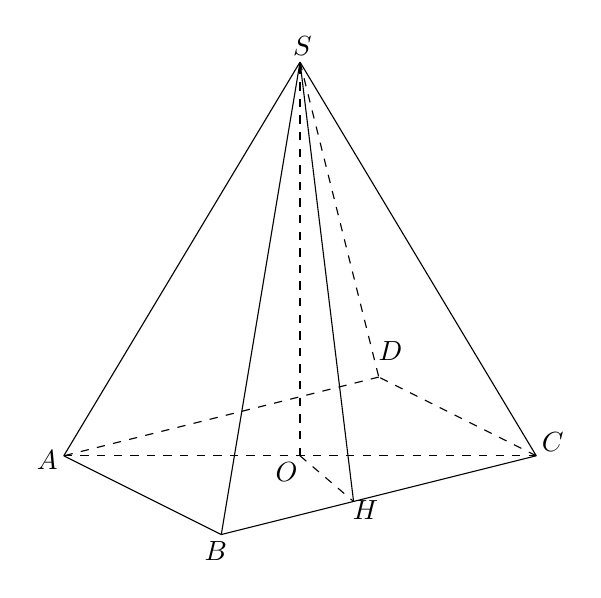
\begin{tikzpicture}
					 \draw (-3,0)-- (-1,-1);
					\draw (-1,-1)--  (3,0);
					\draw  [dashed] (3,0)-- (1,1);
					\draw [dashed]  (1,1)-- (-3,0);
					\draw  (-3,0)-- (0,5);
					\draw (0,5)--  (-1,-1);
					\draw [dashed] (0,0)-- (0,5); 
					\draw [dashed] (0,5)--  (1,1);
					\draw (0,5)-- (3,0); 
					 \draw [dashed] (0,0)-- (0.68,-0.58);
					 \draw (0.68,-0.58)-- (0,5);
					\draw [dashed] (-3,0)-- (3,0); 
					\draw [fill=black] (-3,0); 
					\draw[color=black] (-3.21,-0.05) node  {$A$};
					 \draw [fill=black] (-1,-1);
					\draw[color=black] (-1.07,-1.21)  node {$B$};
					 \draw [fill=black] (3,0);
					\draw[color=black] (3.21,0.17) node {$C$}; 
					\draw [fill=black]  (1,1);
					\draw[color=black]  (1.15,1.33) node {$D$};
					\draw [fill=black] (0,5); 
					 \draw[color=black] (0.03,5.2) node {$S$};
					\draw [fill=black] (0,0); 
					 \draw[color=black] (-0.17,-0.2) node {$O$};
					 \draw [fill=black] (0.68,-0.58);
					\draw[color=black] (0.83,-0.69) node {$H$}; 
				\end{tikzpicture}
		\end{center}
		Gọi $H$  là hình chiếu của $S$ lên $BC$. Ta có $SH \perp BC$ và $OH \perp BC$, suy ra $\widehat{SHO}$ là góc phẳng nhị diện $\left[A, BC, S \right]$.\\
		Ta có $OC=\sqrt{BC^2-OB^2}=\dfrac{a\sqrt{6}}{3}$,  $\dfrac{1}{OH^2}=\dfrac{1}{OB^2}+\dfrac{1}{OC^2}\Rightarrow OH=\dfrac{a\sqrt{2}}{3}$.\\
		Trong tam giác vuông $SHO$ ta có $\tan \widehat{SHO}=\dfrac{SO}{OH}=\sqrt{3}$.\\ 
	Suy ra $\widehat{SHO}=60^\circ$.} 
\end{ex}

% nguồn: Ok_Toan11_TracNghiem_Lan2
\begin{ex}%[1H8H3-3]%[ma:1940915b]
	Cho hình chóp  $S.ABC$ có đáy $ABC$ là tam giác vuông cân tại $A$, $SA \perp (ABC)$.\\
	Góc phẳng nhị  diện $\left[B, SA, C \right]$ có số đo bằng
	 \choice
		 {$30^\circ$}
		 {$45^\circ$}
		{$60^\circ$} 
		 {\True $90^\circ$}
	\loigiai{ 
		\begin{center}
			\begin{tikzpicture}
					\draw [dashed]  (0,0)-- (-1,-1);
					\draw (-1,-1)-- (4,0); 
					\draw [dashed] (4,0)-- (0,0); 
					\draw [dashed]  (0,0)-- (0,4);
					\draw (0,4)-- (-1,-1); 
					\draw (0,4)-- (4,0); 
					\draw [fill=black]  (0,0);
					\draw[color=black] (-0.32,0.15)  node {$A$};
					\draw  [fill=black] (-1,-1);
					\draw[color=black] (-1.16,-1.13) node  {$B$};
					 \draw [fill=black] (4,0);
					\draw[color=black] (4.26,0.15)  node {$C$};
					\draw  [fill=black] (0,4);
					\draw[color=black] (-0.16,4.2)  node {$S$};
				\end{tikzpicture}
		\end{center}
	Ta có $BA \perp SA$ và $CA  \perp SA$, suy ra $\widehat{BAC}$ là góc phẳng nhị diện $\left[B, SA, C \right]$ và bằng $90^\circ$.}
\end{ex}

% nguồn: Ok_Toan11_TracNghiem_Lan2
\begin{ex}%[1H8H3-3]%[ma:4f78d0ee]
	Cho hình chóp $S.ABCD$ có đáy $ABCD$ là hình chữ nhật, tam giác $SAB$ đều và nằm trong mặt phẳng vuông  góc với đáy. Gọi $H, K$ lần lượt là trung điểm của $AB, CD$.\\
	Góc  phẳng nhị diện $\left[S, AB, K \right]$ là
	\choice 
		 {\True $\widehat{SHK}$}
		 {$\widehat{SAK}$}
		 {$\widehat{SAC}$}
		 {$\widehat{SAD}$}
	 \loigiai{
		\begin{center}
			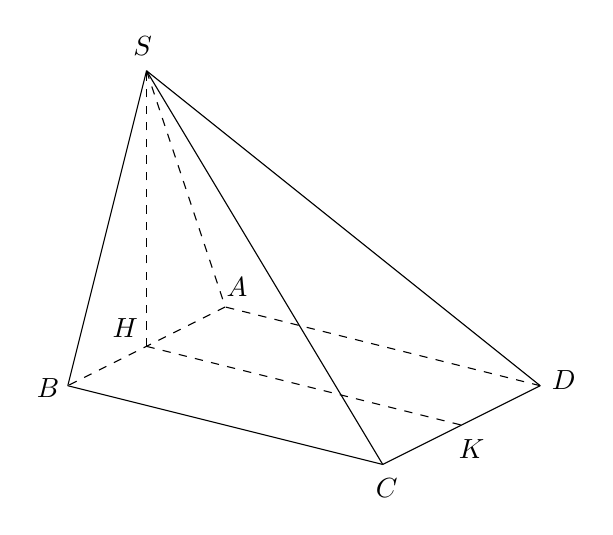
\begin{tikzpicture}
					\draw  [dashed] (0,0)-- (-2,-1);
					 \draw (-2,-1)-- (2,-2);
					\draw  (2,-2)-- (4,-1);
					 \draw [dashed] (4,-1)-- (0,0);
					\draw [dashed] (-1,-0.5)--  (-1,3);
					 \draw (-2,-1)-- (-1,3);
					 \draw [dashed] (-1,3)-- (0,0);
					\draw  (-1,3)-- (4,-1);
					 \draw (2,-2)-- (-1,3);
					\draw [dashed] (-1,-0.5)-- (3,-1.5); 
					\draw [fill=black]  (0,0);
					\draw[color=black]  (0.15,0.25) node {$A$};
					 \draw [fill=black] (-2,-1);
					\draw[color=black]  (-2.25,-1.03) node {$B$};
					\draw  [fill=black] (2,-2);
					\draw[color=black] (2.05,-2.3) node  {$C$};
					\draw [fill=black]  (4,-1);
					\draw[color=black]  (4.3,-0.93) node {$D$};
					 \draw [fill=black] (-1,-0.5);
					\draw[color=black] (-1.27,-0.27)  node {$H$};
					\draw [fill=black]  (-1,3);
					\draw[color=black] (-1.05,3.31) node  {$S$};
					\draw [fill=black]  (3,-1.5);
					\draw[color=black] (3.13,-1.8) node {$K$}; 
				\end{tikzpicture}
		\end{center}
	Ta có $SH \perp AB$ và $KH \perp AB$, suy ra $\widehat{SHK}$ là  góc phẳng nhị diện $\left[S, AB, K \right]$.}
\end{ex}

% nguồn: Ok_Toan11_TracNghiem_Lan2
\begin{ex}%[1H8H3-3]%[ma:f9c23331]
	Cho hình chóp $S.ABC$ có $SA \perp (ABC)$. Gọi $H$ là hình chiếu của $A$ trên $BC$.  Biết $\triangle ABC$ vuông tại $A$, $\widehat{ABC}=30^\circ$, $AC=a$, $SA=\dfrac{a\sqrt{3}}{2}$.\\
	Tính số đo góc nhị diện $\left[S, BC, A  \right]$
	\choice 
		 {$30^\circ$}
		{\True $45^\circ$} 
		{$60^\circ$} 
		 {$75^\circ$}
	\loigiai{ 
		\begin{center}
			\begin{tikzpicture}
					\draw [dashed] (0,0)-- (-1,-1); 
					\draw  (-1,-1)-- (4,0);
					\draw [dashed]  (4,0)-- (0,0);
					\draw [dashed]  (0,0)-- (0,4);
					\draw (0,4)-- (-1,-1); 
					\draw  (0,4)-- (4,0);
					\draw [dashed] (0,0)-- (1.06,-0.59); 
					\draw  (1.06,-0.59)-- (0,4);
					\draw  [fill=black] (0,0);
					\draw[color=black] (-0.32,0.2) node  {$A$};
					 \draw [fill=black] (-1,-1);
					\draw[color=black] (-1.16,-1.13) node  {$B$};
					 \draw [fill=black] (4,0);
					\draw[color=black] (4.26,0.15)  node {$C$};
					\draw [fill=black]  (0,4);
					\draw[color=black] (-0.16,4.2) node {$S$}; 
					\draw  [fill=black] (1.06,-0.59);
					\draw[color=black] (1.2,-0.79) node {$H$}; 
				\end{tikzpicture}
		\end{center}
		Ta  có $SA \perp (ABC) \Rightarrow SA \perp BC$, theo giả thiết $AH \perp BC \Rightarrow BC \perp (SAH)$.\\
		Do đó $\left[S, BC, A \right]=\widehat{SHA}$.\\ 
		Vì tam giác $ABC$ vuông tại $A$ nên $\tan \widehat{ABC}=\dfrac{AC}{AB}  \Rightarrow AB=\dfrac{AC}{\tan 30^\circ}=a\sqrt{3}$.\\
		Khi đó $\dfrac{1}{AH^2}=\dfrac{1}{AB^2}+\dfrac{1}{AC^2}=\dfrac{1}{3a^2}+\dfrac{1}{a^2}=\dfrac{4}{3a^2}\Rightarrow AH=\dfrac{a\sqrt{3}}{2}$.\\ 
	Tam giác $SAH$ vuông tại $A$  có $SA=AH=\dfrac{a\sqrt{3}}{2} \Rightarrow \widehat{SHA}=45^\circ$.}
\end{ex}

% nguồn: Ok_Toan11_TracNghiem_Lan2
\begin{ex}%[1H8H3-3]%[ma:4963cfef]
	Cho hình lập phương $ABCD.A'B'C'D'$, gọi $H$ là hình chiếu của $B$ lên $A'C$.\\ 
	Góc phẳng nhị diện $\left[B, A'C,  D \right]$ là
	 \choice
		{\True $\widehat{BHD}$} 
		{$\widehat{BCD}$} 
		 {$\widehat{BA'D}$}
		{$\widehat{BAD}$} 
	 \loigiai{
		\begin{center}
			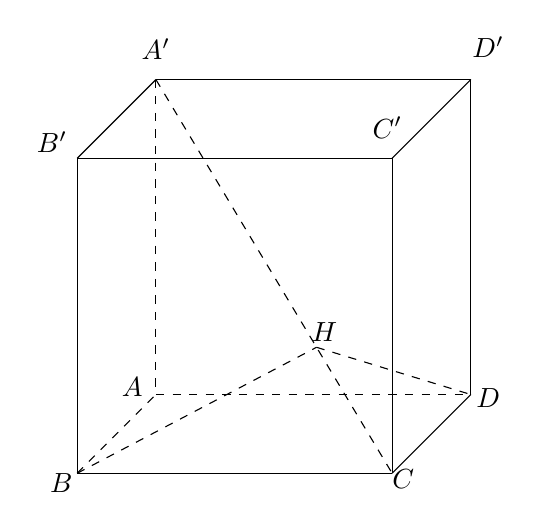
\begin{tikzpicture}
					 \draw (0,4)-- (-1,3);
					\draw  (-1,3)-- (-1,-1);
					\draw  [dashed] (-1,-1)-- (0,0);
					\draw [dashed] (0,0)--  (4,0);
					\draw (4,0)--  (3,-1);
					\draw  (3,-1)-- (-1,-1);
					\draw  (3,-1)-- (3,3);
					\draw  (3,3)-- (-1,3);
					\draw (0,4)--  (4,4);
					 \draw (4,4)-- (3,3);
					\draw  (4,4)-- (4,0);
					\draw [dashed]  (0,4)-- (0,0);
					\draw [dashed]  (0,4)-- (3,-1);
					 \draw [dashed] (-1,-1)-- (2.04,0.60);
					\draw [dashed] (2.04,0.60)--  (4,0);
					\draw  [fill=black] (0,0);
					 \draw[color=black] (-0.3,0.1) node {$A$};
					 \draw [fill=black] (-1,-1);
					\draw[color=black] (-1.2,-1.13) node {$B$}; 
					\draw  [fill=black] (3,-1);
					\draw[color=black] (3.14,-1.07)  node {$C$};
					\draw [fill=black]  (4,0);
					\draw[color=black]  (4.22,-0.05) node {$D$};
					\draw [fill=black] (0,4); 
					\draw[color=black]  (0,4.39) node {$A'$};
					\draw [fill=black]  (-1,3);
					\draw[color=black] (-1.32,3.21) node  {$B'$};
					\draw  [fill=black] (3,3);
					\draw[color=black] (2.94,3.39) node {$C'$}; 
					\draw [fill=black]  (4,4);
					\draw[color=black] (4.22,4.41) node {$D'$}; 
					\draw [fill=black]  (2.04,0.60);
					\draw[color=black] (2.14,0.8) node {$H$}; 
				\end{tikzpicture}
		\end{center}
	Ta có $BH \perp A'C$ và $DH \perp A'C$, suy ra $\widehat{BHD}$ là góc phẳng nhị diện $\left[B, A'C, D  \right]$.}
\end{ex}


%%%%%%%%%%%%%%%% ĐÚNG/SAI %%%%%%%%%%%%%%%%

% nguồn: Ok_dungsai_lop11_Lan2
\begin{ex}%[1H8H3-3]%[ma:d29f6e9c]
	Cho hình chóp $S.ABCD$ có $SA\perp \left(ABCD\right)$, đáy  $ABCD$ là hình chữ nhật tâm $O$, $AB< AD$.
	\choiceTF 
		{$SO$ là hình  chiếu của $SB$ trên $\left(SAC\right)$}
		{\True $\triangle  ABC$ là hình chiếu của $\triangle SBC$ trên $\left(ABCD\right)$}
		{$\triangle SBC$ là hình chiếu của $\triangle  ABC$ trên $\left(SBC\right)$}
		{\True Vẽ $DQ\perp SC$ tại $Q$ với $Q\in SC$, $RQ\perp SC$ tại $Q$  với $R\in BC$, khi đó $DR\perp AC$}
	 \loigiai{
		\begin{itemchoice}
			\itemch 
			Vẽ $BE\perp AC$ tại  $E$, ta có: $\heva{&{BE\perp AC} \\
			&{BE\perp SA} 
			} \Rightarrow BE\perp \left(SAC\right)$ tại $E$, suy ra $E$ là hình chiếu của $B$ trên $\left(SAC\right)$. Do đó $SE$ là hình chiếu của $SB$  trên $\left(SAC\right)$.
			 \itemch
			Ta có $SA\perp \left(ABCD\right)\Rightarrow A$ là hình chiếu của $S$ trên  $\left(ABCD\right)$. Do đó $\triangle ABC$ là hình chiếu của $\triangle SBC$ trên $\left(ABCD\right)$.
			\itemch 
			Vẽ $AH\perp SB$ tại $H$, ta có: $\heva{&{AH\perp  SB} \\
			&{AH\perp BC \left(do BC\perp  \left(SAB\right)\right)}
			} \Rightarrow AH\perp \left(SBC\right)$ tại $H$, suy ra $H$ là hình chiếu của $A$ trên $\left(SBC\right)$. Do đó $\triangle HBC$ là hình chiếu của $\triangle ABC$  trên $\left(SBC\right)$.
			\itemch 
			Ta có $\heva{&{SC\perp  DQ} \\
			&{SC\perp QR} 
			} \Rightarrow SC\perp \left(DQR\right)\Rightarrow SC\perp  DR$. Lại có $A$ là hình chiếu của $S$ trên $\left(ABCD\right)$, do đó $AC$ là hình chiếu của $SC$ trên $\left(ABCD\right)$. Theo định lý 3đường vuông góc suy ra $DR\perp AC$.
		\end{itemchoice}
	 }
\end{ex}

% nguồn: Ok_dungsai_lop11_Lan2
\begin{ex}%[1H8H3-3]%[ma:979332fe]
	Cho  hình chóp $S.ABCD$ có đáy là hình vuông cạnh $a$, $SA\perp (ABCD)$ và $SA=a\sqrt{2}$.
	\choiceTF 
		{\True Góc giữa $SC$ và $(ABCD)$ bằng  $45^\circ$}
		 {Góc giữa $BD$ và mặt phẳng $(SAC)$ bằng $60^\circ$}
		{\True Hình chiếu  của $SB$ trên mặt phẳng $(SAC)$ là $SO$}
		{Gọi $\alpha$ là góc giữa $SC$ và  $(SBD)$. Khi đó $\cos \alpha=\dfrac{2\sqrt{10}}{10}$}
	\loigiai{ 
		\begin{center}
			\begin{tikzpicture}
					 \draw[dashed] (0,0)--(-2,-1);
					 \draw (-2,-1)--(3,-1);
					\draw  (3,-1)--(5,0);
					 \draw[dashed] (5,0)--(0,0);
					\draw[dashed]  (0,0)--(0,4);
					\draw  (0,4)--(-2,-1);
					\draw (3,-1)--(0,4); 
					\draw  (0,4)--(5,0);
					\draw[dashed] (0,0)--(3,-1); 
					 \draw[dashed] (5,0)--(-2,-1);
					 \draw (3,-1)--(1.791,-1.373);
					\draw[dashed]  (1.6666666666666667,-1)--(0,4);
					 \draw (1.791,-1.373)--(1.6666666666666667,-1);
					\node[above left] at (0,0)  {$A$};
					\node[right]  at (5,0) {$B$};
					\node[below right] at  (3,-1) {$C$};
					\node[below  left] at (-2,-1) {$D$};
					\node[above]  at (0,4) {$S$};
					\node[above] at (1.5,-0.5)  {$O$};
					 \node[below right] at (1.791,-1.373) {$H$};
				\end{tikzpicture}
		\end{center}
		\begin{itemchoice}
			\itemch 
			Góc giữa $SC$ và $(ABCD)$  bằng góc giữa $SC$ và $AC$, hay góc $\widehat{SCA}$. \\
			Ta  có $SA=a\sqrt{2}$; $AC=a\sqrt{2} \Rightarrow \tan \widehat{SCA}=\dfrac{SA}{AC}=1\Rightarrow \widehat{SCA}=45^\circ$.
			 \itemch
			Ta có  $BD\perp SA$; $BD\perp AC\Rightarrow BD\perp (SAC)$. \\
			Vậy góc giữa $BD$ và mặt phẳng $(SAC)$ bằng  $90^\circ$.
			\itemch 
			Hình chiếu của $S$ trên  mặt phẳng $(SAC)$ là $S$. \\
			Hình chiếu của $B$ trên mặt phẳng $(SAC)$  là $O$ vì $BD\perp (SAC)$. \\
			Vậy hình chiếu của  $SB$ trên mặt phẳng $(SAC)$ là $SO$.
			 \itemch
			Kẻ $CH\perp SO$. Vì $\widehat{SOC}$ tù  nên $H$ nằm ngoài đoạn $SO$. \\
			Lại có $BD\perp (SAC)\Rightarrow BD\perp  CH\Rightarrow CH\perp (SBD)$. \\
			Vậy hình chiếu của $SC$ trên $(SBD)$ là $SH$. \\ 
			Suy ra  góc giữa $SC$ và $(SBD)$ là $\widehat{CSH}=\widehat{CSO}$. \\
			Có  $OC=\dfrac{a\sqrt{2}}{2}$; $SC=2a$; $SO=\dfrac{a\sqrt{10}}{2}$. \\
			$\cos \alpha=\dfrac{SO^2+SC^2-CO^2}{2.SO.SC}=\dfrac{3\sqrt{10}}{10}$. 
		\end{itemchoice}
	 }
\end{ex}

% nguồn: Ok_dungsai_lop11_Lan2
\begin{ex}%[1H8H3-3]%[ma:c7d69623]
	Cho khối chóp đều $S.ABCD$ có tất cả các cạnh đều bằng $1$. Điểm $O$ là  tâm của hình vuông $ABCD$ (tham khảo hình vẽ)
	\begin{center}
		\begin{tikzpicture}[line cap=round,line join=round,x=1cm,y=1cm]
				\draw (-3,-1)--(2,-1); 
				 \draw (2,-1)--(4,1);
				\draw (-3,-1)--(0,5); 
				\draw (2,-1)--(0,5); 
				\draw  (0,5)--(4,1);
				 \draw[dashed] (4,1)--(-1,1);
				\draw[dashed]  (-1,1)--(-3,-1);
				 \draw[dashed] (0,5)--(-1,1);
				\draw[dashed]  (-1,1)--(2,-1);
				 \draw[dashed] (4,1)--(-3,-1);
				\node[below left] at (-3,-1)  {$A$};
				\node[below] at (2,-1) {$B$}; 
				 \node[right] at (4,1) {$C$};
				\node[left]  at (-1,1) {$D$};
				 \node[above] at (0,5) {$S$};
				\node[below] at (0.5,0) {$O$}; 
			\end{tikzpicture}
	\end{center}
	Cho biết tính đúng sai của  các khẳng định sau:
	 \choiceTF
		{\True $(SO, (ABCD))=90^\circ$} 
		{$(SB, (ABCD))=60^\circ$} 
		 {\True $(CD, (SBD))=45^\circ$}
		{$(CS, (SBD))=30^\circ$} 
	 \loigiai{
		\begin{center}
			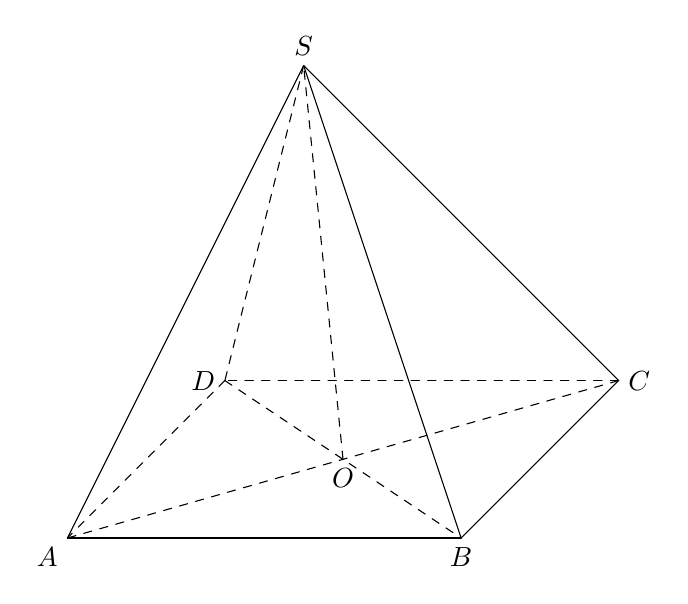
\begin{tikzpicture}[line cap=round,line join=round,x=1cm,y=1cm]
					\draw  (-3,-1)--(2,-1);
					\draw  (2,-1)--(4,1);
					\draw (-3,-1)--(0,5); 
					\draw (2,-1)--(0,5); 
					 \draw (0,5)--(4,1);
					 \draw[dashed] (4,1)--(-1,1);
					\draw[dashed] (-1,1)--(-3,-1); 
					 \draw[dashed] (0,5)--(-1,1);
					\draw[dashed]  (-1,1)--(2,-1);
					\draw[dashed] (4,1)--(-3,-1); 
					\draw[dashed] (0.5,0)--(0,5); 
					\node[below left] at  (-3,-1) {$A$};
					\node[below] at (2,-1)  {$B$};
					 \node[right] at (4,1) {$C$};
					\node[left] at (-1,1)  {$D$};
					\node[above] at (0,5) {$S$}; 
					 \node[below] at (0.5,0) {$O$};
				\end{tikzpicture}
		\end{center}
		\begin{itemchoice}
			\itemch 
			Ta có $SO$ là trung tuyến của  hai tam giác $SAC$ và $SBD$ cân tại $S$ nên \\
			 $\heva{&SO\perp AC\\
			&SO\perp BD} \Rightarrow SO\perp (ABCD) \Rightarrow (SO, (ABCD))=90^\circ$. 
			\itemch 
			 Vì $SO\perp (ABCD)$ nên $(SB, (ABCD))=\widehat{SBO}=\widehat{SBD}$. \\
			Xét tam giác $SBD$ cân tại $S$ và $BD^2=SB^2+SD^2=2 \Rightarrow \triangle SBD$ vuông cân  tại $S$ $\Rightarrow \widehat{SBD}=45^\circ$. \\
			Do đó $(SB, (ABCD))=45^\circ$. 
			\itemch 
			 Ta có $SO\perp (ABCD) \Rightarrow SO\perp CO$ tại $O$. \\
			Lại có $ABCD$ là hình vuông nên $CO\perp BD$ tại $O$.  \\
			Từ  hai điều trên suy ra $CO\perp (SBD)$ tại $O$, do đó $(CD, (SBD))=\widehat{CDO}=\widehat{CDB}=45^\circ$.
			 \itemch
			 Theo chứng minh trên ta có $CO\perp (SBD)$ tại $O$ nên $(CS, (SBD))=\widehat{CSO}$. \\
			Áp dụng hệ thức lượng  trong tam giác vuông $SOC$ ta được: \\
			$\sin \widehat{CSO}=\dfrac{OC}{SC}=\dfrac{\sqrt{2}}{2}  \Rightarrow \widehat{CSO}=45^\circ$.
		\end{itemchoice}
	 }
\end{ex}

% nguồn: Ok_dungsai_lop11_Lan2
\begin{ex}%[1H8H3-3]%[ma:816adb7a]
	Cho hình chóp $S.ABCD$ có đáy $ABCD$ là hình vuông cạnh $a$, $SH\perp (ABCD)$ với $H$ là trung điểm $AB$. Biết $SBD$ là tam giác cân tại $S$ có $\widehat{ASB}=120^\circ$. 
	\choiceTF 
		 {\True Hình chiếu của $S$ lên mặt phẳng $(ABCD)$ là $H$}
		{Góc giữa $SA$ và  $(ABCD)$ bằng $30^\circ$}
		{Góc  giữa $SC$ và $(ABCD)$ là $\alpha$ thỏa $\tan \alpha=\dfrac{1}{\sqrt{2}}$}
		{\True Góc giữa $SH$ và $(SBD)$ là $\beta$ thỏa $\tan \beta=\dfrac{\sqrt{6}}{2}$} 
	\loigiai{ 
		\begin{center}
			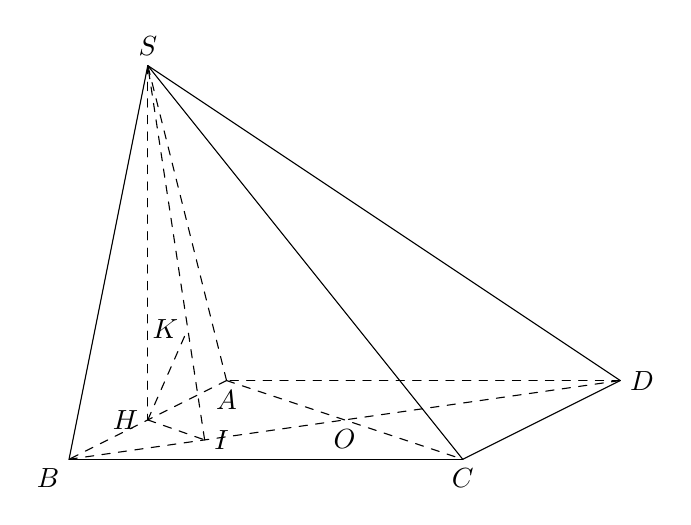
\begin{tikzpicture}[line cap=round,line join=round,x=1cm,y=1cm]
					 \draw[dashed] (0,0)--(-2,-1);
					\draw (-2,-1)--(3,-1); 
					\draw (3,-1)--(5,0); 
					\draw[dashed]  (5,0)--(0,0);
					 \draw[dashed] (0,0)--(-1,4);
					 \draw (-1,4)--(-2,-1);
					 \draw (3,-1)--(-1,4);
					 \draw (-1,4)--(5,0);
					\draw[dashed]  (-2,-1)--(5,0);
					\draw[dashed]  (0,0)--(3,-1);
					 \draw[dashed] (-1,-0.5)--(-0.278,-0.754);
					 \draw[dashed] (-0.278,-0.754)--(-1,4);
					\draw[dashed] (-1,4)--(-1,-0.5); 
					\draw[dashed]  (-1,-0.5)--(-0.492,0.655);
					\node[below] at (0,0)  {$A$};
					\node[below left] at (-2,-1) {$B$}; 
					\node[below]  at (3,-1) {$C$};
					\node[right] at  (5,0) {$D$};
					\node[left]  at (-1,-0.5) {$H$};
					 \node[above] at (-1,4) {$S$};
					\node[right]  at (-0.278,-0.754) {$I$};
					\node[left] at  (-0.492,0.655) {$K$};
					\node[below] at (1.5,-0.5) {$O$}; 
				\end{tikzpicture}
		\end{center}
		\begin{itemchoice}
			 \itemch
			Vì $SH\perp (ABCD)$ nên hình  chiếu của $S$ lên mặt phẳng $(ABCD)$ là $H$.
			 \itemch
			Ta có $(SA, (ABCD))=(SA,AH)=\widehat{SAH}$.  \\
			 Do $\triangle SBD$ cân tại $S$, nên $SB=SD$. \\
			Lại có $H$ là trung điểm của $AB$, $SH \perp AB$. Xét $\triangle SHB$ và $\triangle SHD$,  ta có $SH$ chung, $HB=HD$, vậy $SB=SD$ (đúng với giả thiết). \\
			Trong $\triangle  SAH$, $\widehat{SAH}$ là góc giữa $SA$ và $(ABCD)$. Ta có $SH\perp AB$. \\
			$\widehat{ASB}=120^\circ$. 
			 \itemch
			Ta có $(SC,(ABCD))=(SC,CH)=\widehat{SCH}$.  \\
			Ta có $HC=\sqrt{HB^2+BC^2}=\sqrt{\left(\dfrac{a}{2} \right)^2+a^2}=\dfrac{a\sqrt{5}}{2}$.  \\
			$SH=\dfrac{AH}{\tan\widehat{ASH}}$. 
			\itemch 
			Gọi $O$ là tâm của hình vuông và $I$ là  trung điểm của $BO$. Suy ra $HI\perp BD$. Từ $H$ kẻ $HK\perp SI$ tại $K$. \\
			Ta  có $\heva{&BD\perp HI\\
			&BD\perp SH} \Rightarrow BD\perp (SIH)\Rightarrow BD\perp  HK$. \\
			Ta  có $\heva{&HK\perp SI\\
			 &HK\perp BD} \Rightarrow HK\perp (SBD)\Rightarrow (SH,(SBD))=(SH,SK)=\widehat{HSI}$. \\
			Ta có $HI=\dfrac{1}{2} SO=\dfrac{a\sqrt{2}}{4}$. Xét tam giác $SHI$  có $\tan \widehat{HSI}=\dfrac{HI}{SH}=\dfrac{\dfrac{a\sqrt{2}}{4}}{\dfrac{a\sqrt{3}}{6}}=\dfrac{\sqrt{6}}{2}$. \\
			Vậy góc giữa $SH$ và  $(SBD)$ là $\beta$ thỏa $\tan \beta=\dfrac{\sqrt{6}}{2}$.
		\end{itemchoice}
	 }
\end{ex}

% nguồn: Ok_dungsai_lop11_Lan2
\begin{ex}%[1H8H3-3]%[ma:214ed650]
	Cho hình chóp $S.ABCD$ có đáy $ABCD$ là hình bình hành, $AB=2a$, $BC=a$,  $\widehat{ABC}=120^\circ$. Cạnh bên $SD=a\sqrt{3}$ và $SD$ vuông góc với mặt phẳng đáy.
	 \choiceTF
		{\True  $BD$ là hình chiếu vuông góc của $SB$ trên mặt phẳng $(ABCD)$}
		{  $AC\perp (SBD)$}
		{\True Góc giữa $SA$ và  mặt phẳng $(ABCD)$ bằng $60^\circ$}
		{\True $\sin$ của góc  tạo bởi $SD$ và mặt phẳng $(SAC)$ bằng $\dfrac{\sqrt{2}}{4}$}
	\loigiai{ 
		\begin{center}
			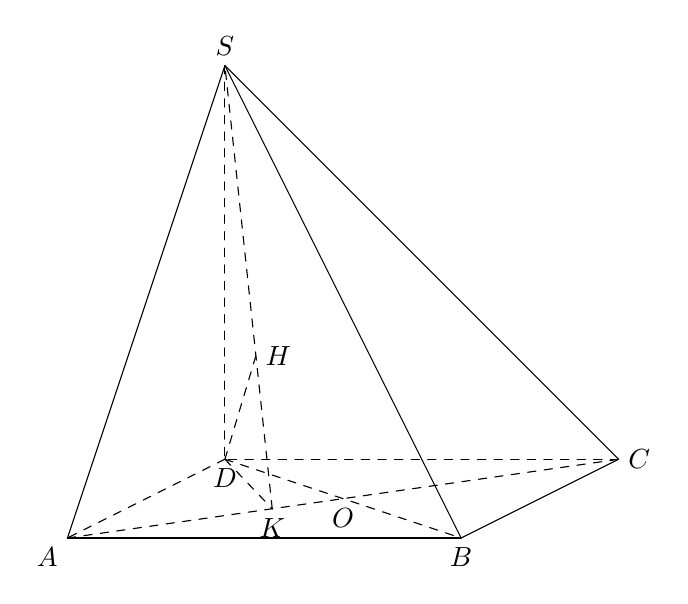
\begin{tikzpicture}[line cap=round,line join=round,x=1cm,y=1cm]
					\draw (-2,-1)--(3,-1); 
					 \draw (3,-1)--(5,0);
					 \draw (-2,-1)--(0,5);
					\draw (0,5)--(3,-1); 
					\draw (0,5)--(5,0); 
					\draw[dashed] (0,5)--(0,0); 
					 \draw[dashed] (0,0)--(-2,-1);
					\draw[dashed] (5,0)--(0,0); 
					\draw[dashed]  (0,0)--(3,-1);
					\draw[dashed] (-2,-1)--(5,0); 
					 \draw[dashed] (0,0)--(0.6012,-0.6284);
					 \draw[dashed] (0.6012,-0.6284)--(0,5);
					\draw[dashed] (0,0)--(0.39361,1.31504); 
					\node[below  left] at (-2,-1) {$A$};
					\node[below] at  (3,-1) {$B$};
					\node[right] at (5,0)  {$C$};
					\node[below]  at (0,0) {$D$};
					\node[above]  at (0,5) {$S$};
					 \node[below] at (1.5,-0.5) {$O$};
					\node[below] at (0.6012,-0.6284)  {$K$};
					\node[right]  at (0.39361,1.31504) {$H$};
				\end{tikzpicture}
		\end{center}
		\begin{itemchoice}
			 \itemch
			Ta có $\heva{&SD\perp (ABCD) \\ 
			 &SB\cap (ABCD)=B} \Rightarrow$ $DB$ là hình chiếu vuông góc của $SB$ trên mặt phẳng $(ABCD)$.
			\itemch 
			Sai vì $AC$ không vuông góc với  $BD$.
			 \itemch
			Ta có $\heva{&SD\perp  (ABCD) \\
			&SA\cap (ABCD)=A} \Rightarrow$ $AD$ là hình chiếu vuông góc của $SA$ trên mặt phẳng $(ABCD)$. \\ 
			Suy ra  góc $\widehat{SAD}$ bằng góc giữa đường thẳng $SA$ và mặt phẳng $(ABCD)$. \\
			$\triangle SDA$ vuông tại  $D$ $\Rightarrow \tan \widehat{SAD}=\dfrac{SD}{AD}=\dfrac{a\sqrt{3}}{a}=\sqrt{3} \Rightarrow \widehat{SAD}=60^\circ$.
			 \itemch
			 Trong $(ABCD)$, từ $D$ kẻ $DK\perp AC$ tại $K$. \\
			Ta có $\heva{&AC\perp DK\\ 
			&AC\perp SD} \Rightarrow AC\perp  (SDK)$. \\
			 Trong $(SDK)$, từ $D$ kẻ $DH\perp SK$ tại $H$. \\
			 Ta có $\heva{&DH\perp SK\\
			&DH\perp AC} \Rightarrow DH\perp  (SAC)$. \\
			Vì $\heva{&DH\perp  (SAC) \\
			&DS\cap (SAC)=S} \Rightarrow$ $SH$ là hình  chiếu vuông góc của $SD$ trên mặt phẳng $(SAC)$. \\
			Suy ra góc  $\widehat{DSH}$ bằng góc giữa đường thẳng $SD$ và mặt phẳng $(SAC)$. \\
			$\triangle SDK$ vuông tại $D$ $\Rightarrow \sin  \widehat{DSK}=\dfrac{DK}{SK}$. \\
			Xét tam giác $ABC$ ta có: \\ $AC=\sqrt{BA^2+BC^2-2BA\cdot BC\cdot\cos \widehat{ABC}}=\sqrt{(2a)^2+a^2-2(2a)a\cos 120^\circ} \\ =\sqrt{4a^2+a^2+2a^2}=a\sqrt{7}$. \\ 
			$S_{\triangle DAC}=\dfrac{1}{2}  DA\cdot DC\cdot\sin \widehat{ADC}=\dfrac{1}{2}\cdot a\cdot 2a\cdot\sin 60^\circ=\dfrac{a^2\sqrt{3}}{2}$. \\
			$S_{\triangle DAC}=\dfrac{1}{2}  DK\cdot AC\Rightarrow \dfrac{a^2\sqrt{3}}{2}=\dfrac{1}{2} DK\cdot a\sqrt{7} \Rightarrow DK=\dfrac{a\sqrt{21}}{7}$. \\
			$SK^2=SD^2+DK^2=\left(a\sqrt{3} \right)^2+\left(\dfrac{a\sqrt{21}}{7} \right)^2=\dfrac{24a^2}{7}  \Rightarrow SK=\dfrac{2a\sqrt{42}}{7}$. \\
			Do  đó $\sin \widehat{DSK}=\dfrac{DK}{SK}=\dfrac{\dfrac{a\sqrt{21}}{7}}{\dfrac{2a\sqrt{42}}{7}}=\dfrac{\sqrt{2}}{4}$.
		\end{itemchoice}
	} 
\end{ex}

% nguồn: Ok_dungsai_lop11_Lan2
\begin{ex}%[1H8H3-3]%[ma:d9ffa242]
	 Cho hình chóp $S.ABCD$ có $SA\perp \left(ABCD\right)$, đáy $ABCD$ là hình vuông tâm $O$.
	\choiceTF 
		{\True $AC$ là hình chiếu của  $SC$ trên $\left(ABCD\right)$}
		{\True  $BD\perp SC$}
		{$C$ là hình chiếu của $B$  trên $\left(SAC\right)$}
		{$\triangle SAB$ là hình chiếu của $\triangle  SAO$ trên $\left(SAB\right)$}
	\loigiai{ 
		\begin{itemchoice}
			\itemch 
			Ta có $SA\perp \left(ABCD\right)\Rightarrow A$ là hình chiếu của $S$ trên $\left(ABCD\right)$. Do  đó $AC$ là hình chiếu của $SC$ trên $\left(ABCD\right)$.
			 \itemch
			Ta có $BD\perp AC$ và $AC$ là hình chiếu của $SC$ trên $\left(ABCD\right)$, suy ra  $BD\perp SC$ (định lý ba đường vuông góc).
			 \itemch
			 $\heva{&{BD\perp AC} \\
			 &{BD\perp SA}
			} \Rightarrow BD\perp \left(SAC\right)$ tại $O$, do đó $O$ là hình chiếu  của $B$ trên $\left(SAC\right)$.
			\itemch 
			Gọi $M$ là trung điểm $AB$ $\Rightarrow OM\perp AB$.\\ 
			 Ta có $\heva{&{OM\perp AB} \\
			&{OM\perp  SA}
			} \Rightarrow OM\perp \left(SAB\right)$ tại $M$.\\ 
			Do đó $M$ là hình chiếu của $O$ trên $\left(SAB\right)$.  Vậy $\triangle SAM$ là hình chiếu của $\triangle SAO$ trên $\left(SAB\right)$.
		\end{itemchoice}
	 }
\end{ex}

% nguồn: Ok_dungsai_lop11_Lan2
\begin{ex}%[1H8H3-3]%[ma:38d11707]
	Cho hình chóp $S.ABCD$ có đáy $ABCD$ là hình vuông  tâm $O$ và các cạnh đều bằng $a$.
	 \choiceTF
		{\True Hình chiếu của $S$ trên mặt  phẳng $(ABCD)$ là $O$}
		{Góc giữa  $SB$ và mặt phẳng $(ABCD)$ là $\widehat{SBA}$}
		{\True Góc giữa $SA$ và mặt phẳng $(SBD)$ bằng  $45^\circ$}
		{\True Gọi $M$ là trung điểm của cạnh $SC$ và $\alpha$ là góc giữa đường thẳng $OM$ và mặt phẳng $(SBC)$. Khi  đó $\sin \alpha=\dfrac{\sqrt{6}}{3}$}
	 \loigiai{
		\begin{center}
			\begin{tikzpicture}[line cap=round,line join=round,>=triangle 45,x=1cm,y=1cm]
					\draw (-3,-1)--(2,-1); 
					\draw (2,-1)--(4,1); 
					\draw (-3,-1)--(0,5); 
					 \draw (2,-1)--(0,5);
					\draw (0,5)--(4,1); 
					 \draw (3,0)--(0,5);
					\draw (2,3)--(2.1106,1.4824); 
					\draw[dashed] (4,1)--(-1,1); 
					\draw[dashed] (-1,1)--(-3,-1); 
					\draw[dashed]  (0,5)--(-1,1);
					\draw[dashed]  (-1,1)--(2,-1);
					\draw[dashed]  (4,1)--(-3,-1);
					 \draw[dashed] (0.5,0)--(0,5);
					\draw[dashed]  (2,3)--(0.5,0);
					 \draw[dashed] (0.5,0)--(3,0);
					\draw[dashed] (2.1106,1.4824)--(0.5,0); 
					\node[below  left] at (-3,-1) {$A$};
					\node[below] at  (2,-1) {$B$};
					 \node[right] at (4,1) {$C$};
					\node[left]  at (-1,1) {$D$};
					\node[above] at  (0,5) {$S$};
					\node[below]  at (0.5,0) {$O$};
					\node[above  right] at (2,3) {$M$};
					\node[below right] at (3,0) {$K$}; 
					\node[right] at (2.1106,1.4824) {$H$}; 
				\end{tikzpicture}
		\end{center}
		\begin{itemchoice}
			 \itemch
			Tam giác $SAC$ cân, $O$ là trung điểm của $AC$  nên $SO\perp AC$. \\
			Chứng minh tương tự ta có $SO\perp  BD$. \\
			Vậy $SO\perp (ABCD)$  hay hình chiếu của $S$ trên mặt phẳng $(ABCD)$ là $O$.
			 \itemch
			Hình  chiếu của $S$ trên mặt phẳng $(ABCD)$ là $O$. \\
			Hình  chiếu của $B$ trên mặt phẳng $(ABCD)$ là $B$. \\
			Hình chiếu  của $SB$ trên mặt phẳng $(ABCD)$ là $OB$. \\
			 Vậy góc giữa $SB$ và mặt phẳng $(ABCD)$ là $\widehat{SBO}$.
			\itemch 
			 Ta có $AO\perp BD$; $AO\perp SO\Rightarrow AO\perp (SBD)$. \\
			Hay hình  chiếu của $A$ trên mặt phẳng $(SBD)$ là $O$. \\
			Hình chiếu của $S$ trên  mặt phẳng $(SBD)$ là $S$. \\
			 Vậy hình chiếu của $SA$ trên mặt phẳng $(SBD)$ là $SO$. \\
			Suy ra góc giữa $SA$ và mặt phẳng $(SBD)$ là góc giữa $SA$ và $SO$ hay $\widehat{ASO}$.  \\
			Có $AC^2=2a^2=a^2+a^2=SA^2+SC^2$  nên tam giác $SAC$ vuông cân tại $S$. \\
			Suy ra  $\widehat{ASO}=\dfrac{1}{2} \widehat{ASC}=45^\circ$.
			\itemch 
			 Kẻ $OK\perp BC$; $OH\perp SK$. \\
			Có $OK\perp BC$; $SO\perp  BC\Rightarrow BC\perp (SOK) \Rightarrow BC\perp OH$. \\
			Mà $OH\perp SK\Rightarrow  OH\perp (SBC)$. \\
			Suy ra $HM$ là hình chiếu vuông góc của $OM$ trên mặt phẳng $(SBC)$. \\ 
			Do đó $\alpha=\widehat{(OM,MH)}=\widehat{OMH}$.  \\
			Lại có $OM=\dfrac{SC}{2}=\dfrac{a}{2}$;  $OK=\dfrac{AB}{2}=\dfrac{a}{2}$; $SO=\dfrac{AC}{2}=\dfrac{a\sqrt{2}}{2}$. \\
			 Khi đó $\dfrac{1}{OH^2}=\dfrac{1}{SO^2}+\dfrac{1}{OK^2}=\dfrac{6}{a^2} \Rightarrow OH=\dfrac{a\sqrt{6}}{6}$. \\
			Vậy $\sin \alpha=\dfrac{OH}{OM}=\dfrac{\sqrt{6}}{3}$. 
		\end{itemchoice}
	} 
\end{ex}

% nguồn: Ok_dungsai_lop11_Lan2
\begin{ex}%[1H8H3-3]%[ma:5e55a839]
	Cho  hình chóp $S.ABCD$ có đáy $ABCD$ là hình vuông cạnh $a$, đường thẳng $SA$ vuông góc với mặt phẳng đáy và $SA=2a$.
	 \choiceTF
		{\True $AC$ hình chiếu  của $SC$ lên mặt phẳng $(ABCD)$}
		{\True $\widehat{(SC;  (ABCD))}=\widehat{SCA}$}
		{ $\widehat{(SB;  (ABCD))}=\widehat{SBA}=45^\circ$}
		{\True Góc giữa đường thẳng $SC$ và mặt phẳng $(ABCD)$ là $\alpha$.  Khi đó $\tan \alpha=\sqrt{2}$}
	 \loigiai{
		\begin{center}
			\begin{tikzpicture}[line cap=round,line join=round,x=1cm,y=1cm]
					 \draw[dashed] (0,5)--(0,0);
					\draw[dashed] (0,0)--(-2,-1); 
					\draw[dashed]  (5,0)--(0,0);
					\draw[dashed] (0,0)--(3,-1); 
					\draw  (-2,-1)--(3,-1);
					\draw (3,-1)--(5,0); 
					\draw (-2,-1)--(0,5); 
					 \draw (0,5)--(3,-1);
					\draw  (0,5)--(5,0);
					\node[below]  at (0,0) {$A$};
					 \node[below left] at (-2,-1) {$B$};
					\node[below] at  (3,-1) {$C$};
					\node[right]  at (5,0) {$D$};
					\node[above] at  (0,5) {$S$};
				\end{tikzpicture}
		\end{center}
		\begin{itemchoice}
			\itemch 
			Ta có: $AC$ là hình chiếu của $SC$ lên mặt phẳng $(ABCD)$. \\ 
			$\widehat{(SC;  (ABCD))}=\widehat{SCA}=\alpha$. \\
			Xét tam giác $SAC$  vuông tại $A$ có: $\tan \widehat{SCA}=\dfrac{SA}{AC}=\dfrac{2a}{a\sqrt{2}}=\sqrt{2}$. \\
			 $\Rightarrow \tan \alpha=\sqrt{2}$.
			\itemch 
			 $\widehat{(SB; (ABCD))}=\widehat{SBA}$. \\
			Xét tam giác $SAB$ vuông tại $A$ có:  $\tan \widehat{SBA}=\dfrac{SA}{AB}=\dfrac{2a}{a}=2$. \\
			$\Rightarrow  \widehat{SBA}\approx 63^\circ 26'$.
		\end{itemchoice}
	} 
\end{ex}

% nguồn: Ok_dungsai_lop11_Lan2
\begin{ex}%[1H8H3-3]%[ma:06e50280]
	Cho hình chóp $S.ABC$ có $SA\perp (ABC)$, tam giác $ABC$ vuông tại  $B$.
	\choiceTF 
		{\True Hình chiếu của $S$ trên  $(ABC)$ là $A$}
		{\True Hình chiếu của $A$ trên mặt phẳng $(SAB)$  là hình chiếu của $A$ trên $SB$}
		{\True Hình chiếu của tam giác  $SBC$ trên mặt phẳng $(ABC)$ là tam giác $ABC$}
		{Hình chiếu của tam giác $SBC$ trên mặt phẳng $(SAB)$ là tam  giác $SAB$}
	\loigiai{ 
		\begin{center}
			\begin{tikzpicture}
					\draw [dashed]  (0,0)-- (-1,-1);
					\draw (-1,-1)--  (4,0);
					\draw [dashed] (4,0)-- (0,0); 
					 \draw [dashed] (0,0)-- (0,4);
					\draw  (0,4)-- (-1,-1);
					\draw (0,4)-- (4,0); 
					 \draw [fill=black] (0,0);
					\draw[color=black]  (-0.32,0.15) node {$A$};
					\draw [fill=black]  (-1,-1);
					\draw[color=black] (-1.16,-1.13) node  {$B$};
					 \draw [fill=black] (4,0);
					\draw[color=black] (4.26,0.15) node  {$C$};
					\draw  [fill=black] (0,4);
					\draw[color=black] (-0.16,4.2)  node {$S$};
				\end{tikzpicture}
		\end{center}
		\begin{itemchoice}
			 \itemch
			Vì $SA\perp (ABC)$. 
			 \itemch
			Kẻ $AH\perp SB$ suy  ra $H$ là hình chiếu của $A$ trên $SB$. \\
			Lại có $\left. \begin{array}{l} BC\perp BA \\ BC\perp SA
	\end{array}\right\}\Rightarrow BC\perp (SAB)\Rightarrow BC\perp AH\Rightarrow AH\perp (SAB)$. \\
	Vậy $H$ là hình chiếu của $A$ trên  $(SAB)$.
	\itemch 
	Hình chiếu của $S$, $B$, $C$ trên  $(ABC)$ lần lượt là $A$, $B$, $C$.
	 \itemch
	Hình chiếu của $S$, $B$ trên mặt phẳng  $(SAB)$ lần lượt là $S$, $B$. \\
	Theo chứng minh trên có $BC\perp (SAB)$ nên hình chiếu của $C$ trên mặt phẳng $(SAB)$ là  $B$. \\
	Vậy hình chiếu của tam giác $SBC$ trên  mặt phẳng $(SAB)$ là tam giác $SAB$.
\end{itemchoice}
 }
\end{ex}

% nguồn: Ok_dungsai_lop11_Lan2
\begin{ex}%[1H8H3-3]%[ma:bf8a53c9]
	Cho hình chóp $S.ABCD$ có đáy $ABCD$ là hình vuông cạnh $a$. Biết $SA$ vuông góc với mặt phẳng $(ABCD)$ và $SA=a\sqrt{2}$. Gọi $H$, $K$ lần  lượt là hình chiếu của $A$ trên $SB$ và $SD$.
	\choiceTF 
		{\True Góc giữa $SD$ và mặt phẳng $(ABCD)$ bằng góc $\widehat{SDA}$} 
		{Góc giữa $SA$ và  mặt phẳng $(SBC)$ bằng góc $\widehat{SCA}$}
		{Góc giữa $SC$ và mặt  phẳng $(ABCD)$ bằng $30^\circ$}
		{\True Góc tạo bởi đường thẳng $SD$ và mặt  phẳng $(AHK)$ bằng $60^\circ$}
	 \loigiai{
		\begin{center}
			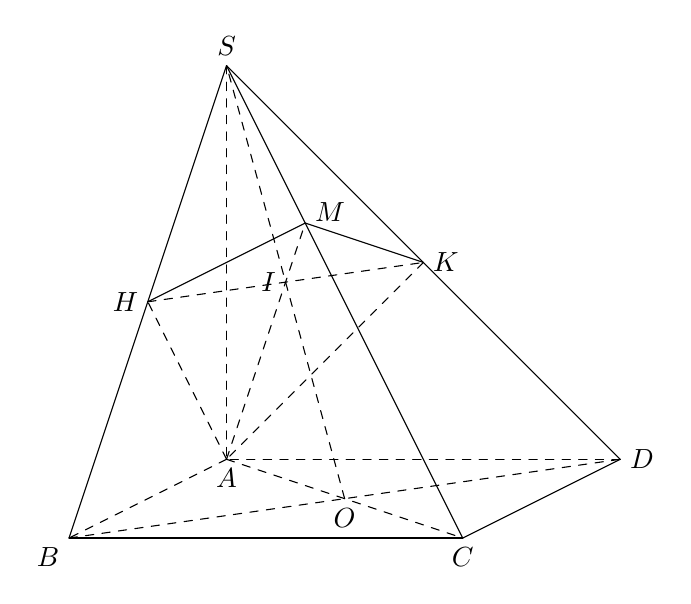
\begin{tikzpicture}[line cap=round,line join=round,x=1cm,y=1cm]
					 \draw[dashed] (0,5)--(0,0);
					 \draw[dashed] (0,0)--(-2,-1);
					 \draw[dashed] (5,0)--(0,0);
					 \draw[dashed] (0,0)--(3,-1);
					\draw[dashed] (-2,-1)--(5,0); 
					 \draw[dashed] (1.5,-0.5)--(0,5);
					\draw[dashed] (-1,2)--(2.5,2.5); 
					 \draw[dashed] (0,0)--(-1,2);
					\draw[dashed]  (2.5,2.5)--(0,0);
					\draw[dashed] (0,0)--(1,3); 
					 \draw (-2,-1)--(3,-1);
					 \draw (3,-1)--(5,0);
					 \draw (-2,-1)--(0,5);
					\draw  (0,5)--(3,-1);
					\draw (0,5)--(5,0); 
					 \draw (-1,2)--(1,3);
					\draw (1,3)--(2.5,2.5); 
					\node[below] at (0,0)  {$A$};
					 \node[below left] at (-2,-1) {$B$};
					\node[below] at (3,-1)  {$C$};
					 \node[right] at (5,0) {$D$};
					\node[above]  at (0,5) {$S$};
					\node[below]  at (1.5,-0.5) {$O$};
					\node[left]  at (-1,2) {$H$};
					\node[right]  at (2.5,2.5) {$K$};
					 \node[left] at (0.75,2.25) {$I$};
					\node[above  right] at (1,2.9) {$M$};
				\end{tikzpicture}
		\end{center}
		\begin{itemchoice}
			\itemch 
			Ta có $\heva{&SA\perp (ABCD) \\ 
			&SD\cap (ABCD)=D} \Rightarrow$ $AD$ là hình chiếu vuông góc của  $SD$ trên mặt phẳng $(ABCD)$. \\
			Suy ra góc giữa đường thẳng $SD$ và mặt phẳng $(ABCD)$ là góc $\widehat{SDA}$. 
			 \itemch
			Ta có $\heva{&BC\perp AB\\ 
			&BC\perp SA} \Rightarrow BC\perp (SAB)$.  \\
			Mà $AH\subset (SAB)$ nên $AH\perp  BC$. \\
			Từ $AH\perp SB$ và $AH\perp BC$, suy  ra $AH\perp (SBC)$. \\
			Do đó, hình chiếu vuông  góc của $SA$ lên $(SBC)$ là $SH$. \\
			 Vậy góc giữa $SA$ và mặt phẳng $(SBC)$ là góc $\widehat{ASH}$.
			 \itemch
			Ta có $\heva{&SA\perp (ABCD)  \\
			&SC\cap (ABCD)=C} \Rightarrow$ $AC$ là hình chiếu vuông góc của $SC$  trên mặt phẳng $(ABCD)$. \\
			Suy ra góc giữa đường thẳng  $SC$ và mặt phẳng $(ABCD)$ là góc $\widehat{SCA}$. \\
			 Xét tam giác $SAC$ vuông tại $A$ có $AC=a\sqrt{2}$. \\
			Ta có  $\tan \widehat{SCA}=\dfrac{SA}{AC}=\dfrac{a\sqrt{2}}{a\sqrt{2}}=1\Rightarrow \widehat{SCA}=45^\circ$.
			\itemch 
			Ta có $AK\perp SD$ và $CD\perp (SAD)$ (vì $CD\perp AD$ và $CD\perp  SA$). \\
			Do $AK\subset  (SAD)$ nên $CD\perp AK$. \\
			Từ $AK\perp SD$  và $AK\perp CD$, suy ra $AK\perp (SCD)$, do đó $AK\perp SC$. \\
			Tương tự, ta có $BC\perp (SAB)$ nên $BC\perp AH$.  Từ $AH\perp SB$ và $AH\perp BC$, suy ra $AH\perp (SBC)$, do đó $AH\perp SC$. \\
			Vì  $AH\perp SC$ và $AK\perp SC$, nên $SC\perp (AHK)$. \\
			Góc giữa đường thẳng $SD$ và mặt  phẳng $(AHK)$ là góc giữa $SD$ và đường thẳng vuông góc với $(AHK)$ tại $S$, đó là đường thẳng $SC$. \\
			Vậy góc  giữa $SD$ và $(AHK)$ là góc $\widehat{DSC}$. \\
			Xét tam giác $DSC$ có $SD=\sqrt{SA^2+AD^2}=\sqrt{(a\sqrt{2})^2+a^2}=a\sqrt{3}$, $SC=\sqrt{SA^2+AC^2}=\sqrt{(a\sqrt{2})^2+(a\sqrt{2})^2}=2a$ và $CD=a$.  \\
			Ta  có:\\
			$\cos\widehat{DSC}=\dfrac{SD^2+SC^2-CD^2}{2\cdot SD\cdot SC}=\dfrac{(a\sqrt{3})^2+(2a)^2-a^2}{2(a\sqrt{3})(2a)}=\dfrac{3a^2+4a^2-a^2}{4a^2\sqrt{3}}=\dfrac{6a^2}{4a^2\sqrt{3}}=\dfrac{3}{2\sqrt{3}}=\dfrac{\sqrt{3}}{2}$. \\ 
			Suy ra $\widehat{DSC}=30^\circ$.  \\
			Góc giữa $SD$  và $(AHK)$ là $90^\circ-\widehat{DSC}=90^\circ-30^\circ=60^\circ$.
		\end{itemchoice}
	} 
\end{ex}

% nguồn: Ok_dungsai_lop11_Lan2
\begin{ex}%[1H8H3-3]%[ma:0f32763e]
	Cho hình chóp $S.ABCD$ có $ABCD$ là hình vuông, $O$ là giao điểm  của hai đường chéo và $SA\perp (ABCD)$. Xét tính đúng sai của các mệnh đề sau:
	\choiceTF 
		{\True Hình chiếu của $S$  trên $(ABCD)$ là $A$}
		{Hình chiếu của $A$  trên $(SBC)$ là $B$}
		{Hình chiếu của tam giác $SBC$ trên  $(ABCD)$ là tam giác $OBC$}
		{Hình chiếu của tam  giác $SOB$ trên $(SAB)$ là tam giác $SAB$}
	\loigiai{ 
		\begin{center}
			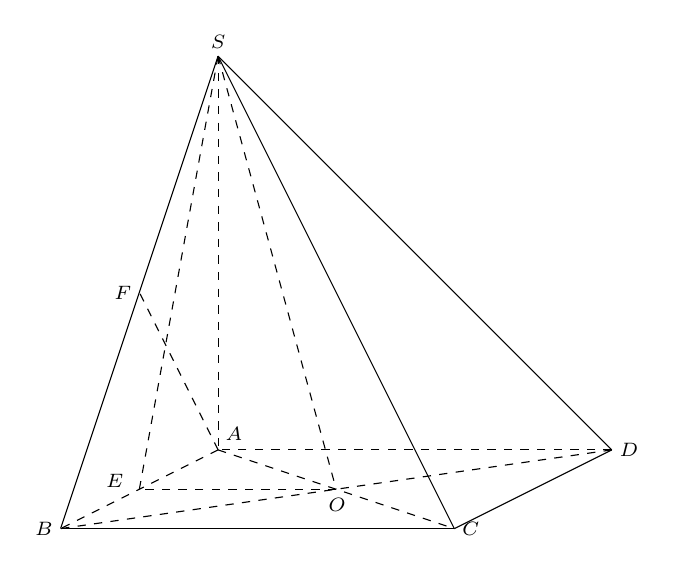
\begin{tikzpicture}
					 \draw [dashed] (0,5)-- (0,0);
					\draw [dashed] (0,0)-- (-2,-1); 
					\draw  (-2,-1)-- (3,-1);
					\draw  (3,-1)-- (5,0);
					 \draw [dashed] (5,0)-- (0,0);
					\draw (-2,-1)--  (0,5);
					\draw (0,5)--  (3,-1);
					 \draw (0,5)-- (5,0);
					\draw [dashed] (0,0)-- (3,-1); 
					 \draw [dashed] (5,0)-- (-2,-1);
					\draw [dashed] (0,5)-- (1.5,-0.5); 
					\draw [dashed] (1.5,-0.5)-- (-1,-0.5); 
					\draw  [dashed] (-1,-0.5)-- (0,5);
					\draw [dashed]  (0,0)-- (-1,2);
					\begin{scriptsize}
						\draw [fill=black] (0.2,0.2) node {$A$}; 
						\draw  [fill=black] (-2,-1) node[left] {$B$};
						\draw [fill=black]  (3,-1) node[right] {$C$};
						\draw [fill=black] (5,0) node[right]  {$D$};
						\draw [fill=black] (0,5) node[above] {$S$}; 
						\draw [fill=black] (1.3,-0.7) node[right]  {$O$};
						\draw [fill=black] (-1.1,-0.4) node[left]  {$E$};
						\draw [fill=black]  (-1,2) node[left] {$F$};
					\end{scriptsize}
				\end{tikzpicture}
		\end{center}
		\begin{itemchoice}
			 \itemch
			Vì $SA\perp (ABCD)$ nên $A$ là hình chiếu của $S$ trên $(ABCD)$. 
			\itemch 
			Ta  có $\heva{&BC\perp AB\\
			&BC\perp SA\\ 
			&SA\cap  AB=A} \Rightarrow BC\perp (SAB)$. \\
			Trong  $(SAB)$, vẽ $AF\perp SB$. \\
			 Ta có $\heva{&AF\perp SB\\
			&AF\perp  BC\\
			 &SB\cap BC=B} \Rightarrow AF\perp (SBC)$. \\
			 Vậy hình chiếu của $A$ lên $(SBC)$ là $F$ với $F$ là hình chiếu của $A$ lên $SB$.
			\itemch 
			 Vì $SA\perp (ABCD)$ nên $A$ là hình chiếu của $S$ trên $(ABCD)$. \\
			Mà hình chiếu của $B$ lên $(ABCD)$ là $B$,  hình chiếu của $C$ lên $(ABCD)$ là $C$. \\
			Vậy  hình chiếu của tam giác $SBC$ trên $(ABCD)$ là tam giác $ABC$.
			\itemch 
			Gọi $E$ là trung điểm  của $AB$. \\
			Vì $E$  là trung điểm của $AB$ và $O$ là trung điểm của $AC$ nên $OE\parallel BC\Leftrightarrow OE\perp AB$. \\
			 Ta có $\heva{&OE\perp AB\\
			 &OE\perp SA\\
			&SA\cap AB=A} \Rightarrow OE\perp (SAB)$. \\ 
			Vậy hình  chiếu của $O$ lên $(SAB)$ là $E$. \\
			Mà hình chiếu của $B$ lên $(SAB)$ là $B$, hình  chiếu của $S$ lên $(SAB)$ là $S$. \\
			Do đó, hình chiếu của tam giác $SOB$ trên $(SAB)$ là tam giác  $SEB$.
		\end{itemchoice}
	 }
\end{ex}

% nguồn: Ok_dungsai_lop11_Lan2
\begin{ex}%[1H8H3-3]%[ma:08f66cff]
	Cho hình chóp $S.ABCD$ có đáy $ABCD$ là hình thoi tâm $O$ cạnh $a$, $BD=a$, cạnh $SO\perp (ABCD)$. $M$ và $N$ lần  lượt là trung điểm của các cạnh $BC$ và $SD$. Đường thẳng $MN$ tạo với mặt phẳng $(ABCD)$ một góc $45^\circ$.
	\choiceTF 
		 { $BC\perp (SAB)$}
		{\True $SO$ là hình  chiếu vuông góc của $SB$ trên mặt phẳng $(SAC)$}
		{\True Góc giữa $SB$ và mặt phẳng  $(ABCD)$ bằng góc $\widehat{SBO}$}
		{Gọi $\alpha$ là  góc giữa đường thẳng $MN$ và mặt phẳng $(SAC)$. Khi đó $\sin \alpha=\dfrac{\sqrt{7}}{28}$}
	 \loigiai{
		\begin{center}
			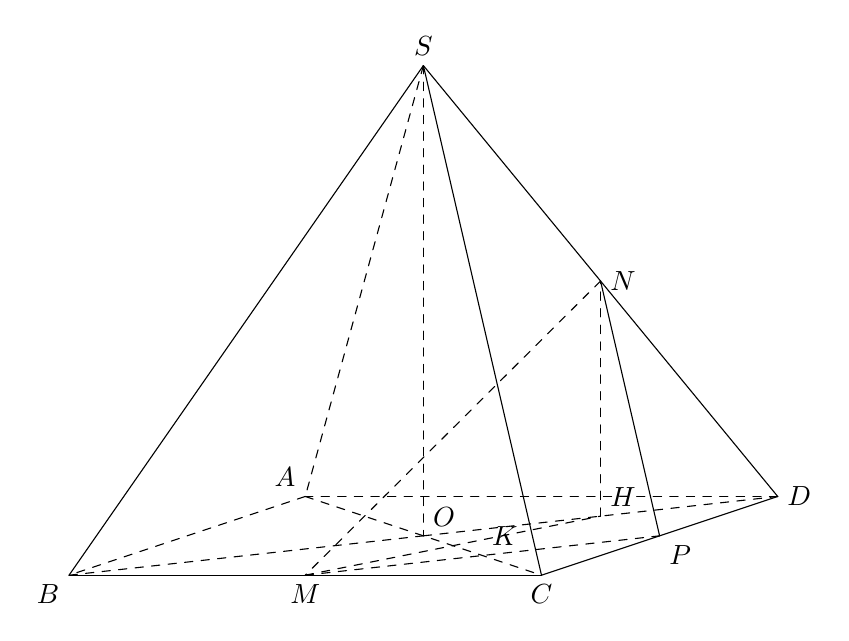
\begin{tikzpicture}[line cap=round,line join=round,x=1cm,y=1cm]
					 \draw (-4,0)--(2,0);
					\draw (2,0)--(5,1); 
					\draw  (0.5,6.472231404958677)--(-4,0);
					 \draw (2,0)--(0.5,6.472231404958677);
					\draw  (0.5,6.472231404958677)--(5,1);
					\draw (3.5,0.5)--(2.75,3.7361157024793386); 
					\draw[dashed] (5,1)--(-1,1); 
					\draw[dashed]  (-1,1)--(-4,0);
					 \draw[dashed] (-1,1)--(2,0);
					\draw[dashed]  (0.5,6.472231404958677)--(-1,1);
					\draw[dashed]  (0.5,6.472231404958677)--(0.5,0.5);
					 \draw[dashed] (0.5,0.5)--(5,1);
					\draw[dashed]  (-4,0)--(0.5,0.5);
					 \draw[dashed] (-1,0)--(2.75,0.75);
					 \draw[dashed] (2.75,0.75)--(2.75,3.7361157024793386);
					\draw[dashed]  (2.75,3.7361157024793386)--(-1,0);
					\draw[dashed] (-1,0)--(3.5,0.5); 
					 \node[below left] at (-4,0) {$B$};
					\node[below] at (2,0)  {$C$};
					 \node[right] at (5,1) {$D$};
					\node[above left] at (-1,1)  {$A$};
					\node[above] at  (0.5,6.472231404958677) {$S$};
					\node[above right]at (0.5,0.5) {$O$}; 
					\node[below] at (-1,0) {$M$}; 
					\node[below  right]at (3.5,0.5){$P$};
					\node[above right]at (2.75,0.75){$H$}; 
					\node[right] at (2.75,3.7361157024793386)  {$N$};
					\node[above right]at (1.25,0.25) {$K$}; 
				\end{tikzpicture}
		\end{center}
		\begin{itemchoice}
			\itemch 
			Trong hình thoi $ABCD$, $BC$ không vuông góc với $AB$ (vì $\widehat{ABC}=120^\circ$) nên $BC$ không vuông  góc với mặt phẳng $(SAB)$.
			 \itemch
			Ta có $\heva{&BD\perp  AC\\
			&BD\perp SO} \Rightarrow BD\perp (SAC)$.  \\
			Vì $BO\subset BD$ nên $BO\perp (SAC)$. Do đó,  $O$ là hình chiếu vuông góc của $B$ lên mặt phẳng $(SAC)$. \\
			Vì $S\in (SAC)$, nên $S$ là hình chiếu vuông  góc của $S$ lên mặt phẳng $(SAC)$. \\
			 Suy ra $SO$ là hình chiếu vuông góc của $SB$ trên mặt phẳng $(SAC)$.
			 \itemch
			Ta có $\heva{&SO\perp (ABCD)  \\
			&SB\cap (ABCD)=B} \Rightarrow$ $OB$ là hình chiếu vuông góc  của $SB$ trên mặt phẳng $(ABCD)$. \\
			Góc giữa đường thẳng $SB$ và mặt phẳng  $(ABCD)$ bằng góc giữa $SB$ và $OB$, chính là góc $\widehat{SBO}$.
			\itemch 
			Gọi  $H$ là trung điểm của $OD$. \\
			Khi đó $NH \parallel SO$.  \\
			Suy ra $NH \bot (ABCD)$ và $\widehat{NMH}  = 45^{\circ}$. \\
			 Xét $\Delta BMH$ ta có $BH = \frac{3a}{4}$, $BM = \frac{a}{2}$, $\widehat{MBH} = 60^{\circ}$. \\
			Do đó $MH = \sqrt{BM^2 + BH^2 - 2BM \cdot BH \cdot \cos 60^{\circ}} = \sqrt{\frac{a^2}{4} + \frac{9a^2}{16} - 2 \cdot  \frac{a}{2} \cdot \frac{3a}{4} \cdot \frac{1}{2}} = \frac{a\sqrt{7}}{4}$. \\
			Do  $\Delta MHN$ vuông cân tại $H$ nên $HN = \frac{a\sqrt{7}}{4}$, $MN = \frac{a\sqrt{14}}{4}$. \\
			Kẻ $MK$ vuông góc với  $OC$ tại $K$, $MK \cap CD = P$. \\
			Suy ra $K$, $P$ lần lượt là trung  điểm của $OC$, $CD$ và $MK \bot (SAC)$. \\
			Do vậy $\sin \alpha = \cos \widehat{NMK} = \cos  \widehat{NMP}$. \\
			Từ $MK \bot (SAC)$ ta có  $MK \bot SC$. \\
			Mặt khác $NP \parallel SC$. \\ 
			Suy ra $MK \bot NP$ hay $MP \bot NP$.  \\
			Do đó $\sin  \alpha = \frac{MP}{MN} = \frac{\frac{a}{2}}{\frac{a\sqrt{14}}{4}} = \frac{\sqrt{14}}{7}$. \\
		\end{itemchoice}
	 }
\end{ex}

% nguồn: Ok_dungsai_lop11_Lan2
\begin{ex}%[1H8H3-3]%[ma:77ba356d]
	Cho hình chóp $S.ABCD$ có đáy $ABCD$ là hình vuông cạnh $a$.  Cạnh bên $SA$ vuông góc với $(ABCD)$ và $SA=a\sqrt{6}$. Hãy xác định tính đúng sai của mỗi mệnh đề dưới đây:
	 \choiceTF
		 {\True $\tan (SC, (ABCD))=\sqrt{3}$}
		{ $\tan (SC,  (SAB))=\sqrt{7}$}
		{ $\sin  (SB, (SAC))=\dfrac{\sqrt{14}}{7}$}
		{\True $\sin (AC, (SBC))=\dfrac{\sqrt{21}}{7}$} 
	 \loigiai{
		\begin{center}
			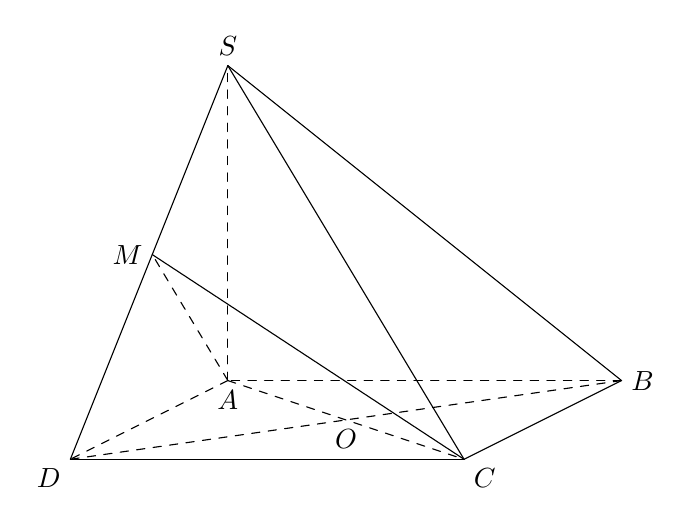
\begin{tikzpicture}[line cap=round,line join=round,x=1cm,y=1cm]
					\draw[dashed]  (0,0)--(-2,-1);
					\draw[dashed]  (5,0)--(0,0);
					\draw[dashed]  (0,0)--(0,4);
					 \draw[dashed] (0,0)--(3,-1);
					\draw[dashed]  (5,0)--(-2,-1);
					 \draw[dashed] (0,0)--(-0.96,1.60);
					 \draw (-2,-1)--(3,-1);
					\draw (3,-1)--(5,0); 
					\draw (0,4)--(-2,-1); 
					 \draw (3,-1)--(0,4);
					\draw (0,4)--(5,0); 
					\draw  (-0.96,1.60)--(3,-1);
					\node[below]  at (0,0) {$A$};
					\node[right] at (5,0)  {$B$};
					\node[below right] at (3,-1) {$C$}; 
					\node[below  left] at (-2,-1) {$D$};
					\node[above]  at (0,4) {$S$};
					\node[below] at  (1.5,-0.5) {$O$};
					\node[left]  at (-0.96,1.60) {$M$};
				\end{tikzpicture}
		\end{center}
		\begin{itemchoice}
			\itemch 
			Vì  $AC$ là hình chiếu vuông góc của $SC$ lên $(ABCD)$ nên $(SC, (ABCD))=\widehat{SCA}$. \\
			Trong tam giác $SCA$, ta có: $\tan \widehat{SCA}=\dfrac{SA}{AC}=\dfrac{a\sqrt{6}}{a\sqrt{2}}=\sqrt{3}$. 
			\itemch 
			Vì $BC\perp (SAB)$ tại $B$ nên $SB$ là hình chiếu vuông góc của  $SC$ lên $(SAB)$. \\
			Do đó $\left(SC,(SAB)\right)=(SC,SB)=\widehat{CSB}$.  \\
			Áp dụng định lí Pytago trong tam giác vuông $SAB$ ta  có: \\
			$SB=\sqrt{SA^2+AB^2}=\sqrt{(a\sqrt{6})^2+a^2}=a\sqrt{7}$.  \\
			Trong tam giác $SCB$, ta có:  $\tan \widehat{CSB}=\dfrac{BC}{SB}=\dfrac{a}{a\sqrt{7}}=\dfrac{\sqrt{7}}{7}$.
			 \itemch
			Vì  $BO\perp (SAC)$ tại $O$ nên $SO$ là hình chiếu vuông góc của $SB$ lên $(SAC)$. \\
			Do đó  $\left(SB,(SAC)\right)=(SB,SO)=\widehat{BSO}$. \\
			 Trong tam giác $SBO$, ta có: $\sin \widehat{BSO}=\dfrac{BO}{SB}=\dfrac{\dfrac{a\sqrt{2}}{2}}{a\sqrt{7}}=\dfrac{\sqrt{14}}{14}$.
			\itemch 
			Gọi $M$ là hình chiếu vuông góc của $A$ lên $SB$. \\ 
			Khi đó  $AM\perp SB$ và $AM\perp BC$ (vì $BC\perp (SAB)$ và $AM\subset (SAB)$) nên $AM\perp (SBC)$ tại $M$. \\
			Do đó $MC$ là hình chiếu vuông góc của $AC$ lên  $(SBC)\Rightarrow (AC,(SBC))=(AC,MC)=\widehat{ACM}$. \\
			 Trong tam giác $SAB$, ta có: $AM=\dfrac{SA\cdot AB}{SB}=\dfrac{a\sqrt{6}\cdot a}{a\sqrt{7}}=\dfrac{a\sqrt{42}}{7}$. \\
			Xét tam giác $ACM$, ta  có: $\sin \widehat{ACM}=\dfrac{MA}{AC}=\dfrac{\dfrac{a\sqrt{42}}{7}}{a\sqrt{2}}=\dfrac{\sqrt{21}}{7}$.
		\end{itemchoice}
	} 
\end{ex}

% nguồn: Ok_dungsai_lop11_Lan2
\begin{ex}%[1H8H3-3]%[ma:dec9baf2]
	Cho hình chóp tam giác đều $S.ABC$ có cạnh đáy bằng $a\sqrt{3}$, cạnh bên bằng $2a$. Gọi $M$ là trung  điểm của $BC$. Khi đó:
	\choiceTF 
		{\True $SO\perp (ABC)$. Trong đó $O$ là tâm đường  tròn ngoại tiếp $\triangle ABC$}
		{\True $\widehat{(SA;(ABC))}=\widehat{(SA;OA)}$} 
		{  $SO=a\sqrt{2}$}
		{Góc giữa đường thẳng $SM$ và mặt phẳng $(ABC)$ là $\alpha$.  Khi đó $\tan \alpha=3\sqrt{2}$}
	 \loigiai{
		\begin{center}
			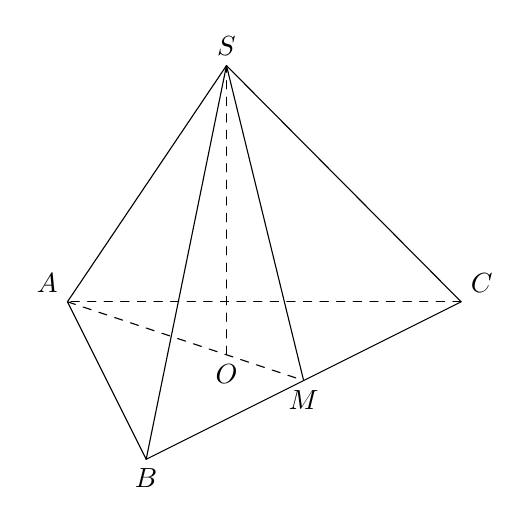
\begin{tikzpicture}[line cap=round,line join=round,x=1cm,y=1cm]
					\draw (-1,0)--(0,-2); 
					 \draw (0,-2)--(4,0);
					\draw  (-1,0)--(1.02,3);
					\draw  (1.02,3)--(0,-2);
					\draw  (1.02,3)--(2,-1);
					\draw  (4,0)--(1.02,3);
					 \draw[dashed] (4,0)--(-1,0);
					 \draw[dashed] (-1,0)--(2,-1);
					\draw[dashed]  (1.02,-0.67)--(1.02,3);
					\node[above left] at  (-1,0) {$A$};
					\node[below] at (0,-2) {$B$}; 
					\node[above  right] at (4,0) {$C$};
					 \node[below] at (2,-1) {$M$};
					\node[below] at (1.02,-0.67) {$O$}; 
					\node[above]  at (1.02,3) {$S$};
				\end{tikzpicture}
		\end{center}
		\begin{itemchoice}
			\itemch 
			Gọi $O$ là tâm đường  tròn ngoại tiếp $\triangle ABC$ đều. \\
			Vì $S.ABC$ là hình chóp tam giác đều nên  $SO\perp (ABC)$.
			 \itemch
			Ta có: $OA$ là  hình chiếu của $SA$ lên mặt phẳng $(ABC)$. \\
			 $\widehat{(SA; (ABC))}=\widehat{(SA; OA)}$.
			 \itemch
			$M$  là trung điểm của $BC$. Khi đó $AM$ là đường trung tuyến đồng thời là đường cao trong $\triangle ABC$ đều $\Rightarrow AM=\dfrac{a\sqrt{3}\cdot\sqrt{3}}{2}=\dfrac{3a}{2}$. \\
			$\Rightarrow  OA=\dfrac{2}{3} AM=\dfrac{2}{3}\cdot\dfrac{3a}{2}=a$. \\
			 $SO=\sqrt{SA^2-OA^2}=\sqrt{(2a)^2-a^2}=a\sqrt{3}$.
			 \itemch
			Ta có: $OM$ là hình chiếu  của $SM$ lên mặt phẳng $(ABC)$. \\
			 $\widehat{(SM; (ABC))}=\widehat{SMO}$. \\
			Xét  tam giác $ABC$ đều, $O$ là trọng tâm nên $OM=\dfrac{1}{3}AM=\dfrac{1}{3}\cdot\dfrac{3a}{2}=\dfrac{a}{2}$. \\
			Xét tam giác $SMO$  vuông tại $O$ có: $\tan \widehat{SMO}=\dfrac{SO}{OM}=\dfrac{a\sqrt{3}}{a/2}=2\sqrt{3}$.
		\end{itemchoice}
	} 
\end{ex}

% nguồn: Ok_dungsai_lop11_Lan2
\begin{ex}%[1H8H3-3]%[ma:7cb7c2e2]
	Cho hình chóp $S.ABCD$  có đáy $ABCD$ là hình vuông cạnh $a$; $SA\perp (ABCD)$ và $SA=a\sqrt{2}$. Gọi $M$ là trung điểm $SB$.
	\choiceTF 
		{ $A$ là hình chiếu vuông góc của $C$  trên mặt phẳng $(SAD)$}
		{\True $AB$ là hình chiếu  vuông góc của $SB$ trên mặt phẳng $(ABCD)$}
		{Góc giữa đường thẳng $SC$ và  mặt phẳng $(ABCD)$ bằng $60^\circ$}
		 {\True Tan của góc giữa đường thẳng $MD$ và mặt phẳng $(ABCD)$ bằng $\dfrac{\sqrt{10}}{5}$}
	 \loigiai{
		\begin{center}
			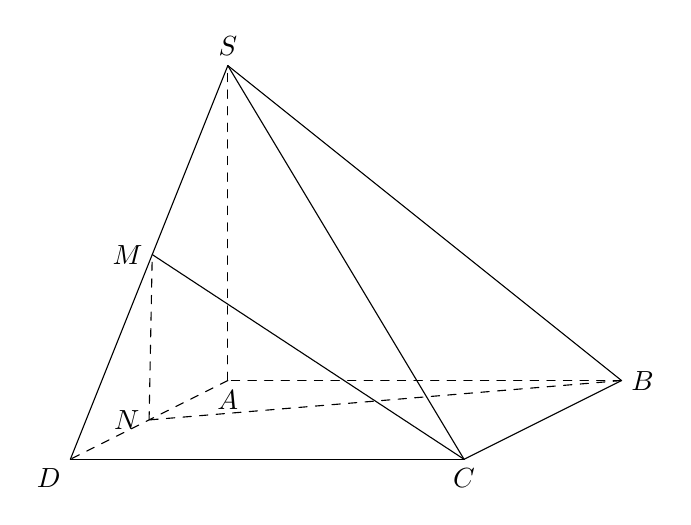
\begin{tikzpicture}[line cap=round,line join=round,x=1cm,y=1cm]
					 \draw[dashed] (0,0)--(-2,-1);
					\draw  (-2,-1)--(3,-1);
					\draw  (3,-1)--(5,0);
					 \draw[dashed] (5,0)--(0,0);
					\draw[dashed] (0,0)--(0,4); 
					\draw (0,4)--(-2,-1); 
					\draw  (3,-1)--(0,4);
					\draw (0,4)--(5,0); 
					\draw (-0.96,1.60)--(3,-1); 
					\draw[dashed] (5,0)--(-1,-0.5); 
					\draw[dashed]  (-1,-0.5)--(-0.96,1.60);
					 \node[below] at (0,0) {$A$};
					\node[right] at (5,0) {$B$}; 
					\node[below] at (3,-1)  {$C$};
					 \node[below left] at (-2,-1) {$D$};
					\node[above]  at (0,4) {$S$};
					\node[left]  at (-0.96,1.60) {$M$};
					\node[left] at (-1,-0.5)  {$N$};
				\end{tikzpicture}
		\end{center}
		\begin{itemchoice}
			 \itemch
			Giả sử $A$ là hình chiếu vuông góc của $C$ trên mặt phẳng $(SAD)$ khi đó $AC\perp (SAD)$. \\ 
			Mặt khác $\heva{&DC\perp AD\\ 
			&SA\perp (ABCD)} \Rightarrow DC\perp SA \Rightarrow DC\perp (SAD)$.  \\
			Suy ra $AC\equiv DC$  (vô lí).
			\itemch 
			 Ta có $\heva{&SA\perp (ABCD) \\
			&SB\cap (ABCD)=B} \Rightarrow$  $AB$ là hình chiếu vuông góc của $SB$ trên mặt phẳng $(ABCD)$.
			 \itemch
			Ta có  $\heva{&SA\perp (ABCD) \\
			&SC\cap (ABCD)=C} \Rightarrow$ $AC$ là  hình chiếu vuông góc của $SC$ trên mặt phẳng $(ABCD)$. \\
			Suy ra góc giữa đường thẳng $SC$ và  mặt phẳng $(ABCD)$ là góc $\widehat{SCA}$. \\
			Trong $\triangle SAC$  vuông tại $A$ có $AC=a\sqrt{2}$. \\
			 Ta có $\tan\widehat{SCA}=\dfrac{SA}{AC}=\dfrac{a\sqrt{2}}{a\sqrt{2}}=1\Rightarrow \widehat{SCA}=45^\circ$.
			\itemch 
			Gọi $N$ là trung điểm  của $AB$. \\
			Ta có $MN$ là đường trung bình của $\triangle SAB$ nên  $MN\parallel SA$ và $MN=\dfrac{1}{2} SA=\dfrac{a\sqrt{2}}{2}$. \\
			Mà  $SA\perp (ABCD)\Rightarrow MN\perp (ABCD)$. \\
			 Ta có $\heva{&MN\perp (ABCD) \\
			&MD\cap (ABCD)=D} \Rightarrow$ $ND$ là hình chiếu vuông  góc của $MD$ trên mặt phẳng $(ABCD)$. \\
			Suy ra góc giữa  $MD$ và mặt phẳng $(ABCD)$ là góc $\widehat{MDN}$. \\
			Ta có $DN=\sqrt{AD^2+AN^2}=\sqrt{a^2+\left(\dfrac{a}{2}\right)^2}=\sqrt{a^2+\dfrac{a^2}{4}}=\dfrac{a\sqrt{5}}{2}$.  \\
			Xét $\triangle MND$ vuông tại $N$, có $\tan  \widehat{MDN}=\dfrac{MN}{DN}=\dfrac{\dfrac{a\sqrt{2}}{2}}{\dfrac{a\sqrt{5}}{2}}=\dfrac{\sqrt{2}}{\sqrt{5}}=\dfrac{\sqrt{10}}{5}$.
		\end{itemchoice}
	} 
\end{ex}

% nguồn: Ok_dungsai_lop11_Lan2
\begin{ex}%[1H8H3-3]%[ma:11b73976]
	Cho hình chóp $S.ABC$ có $SA\perp  \left(ABC\right)$, tam giác $ABC$ là tam giác đều.
	 \choiceTF
		{\True Hình chiếu của  $S$ trên $\left(ABC\right)$ là $A$}
		{Hình chiếu của $C$  trên $\left(SAB\right)$ là $A$}
		{\True Hình  chiếu của tam giác $SBC$ trên $\left(ABC\right)$ là tam giác $ABC$}
		{Hình chiếu của tam giác  $SBC$ trên $\left(SAB\right)$ là tam giác $SAB$}
	\loigiai{ 
		\begin{center}
			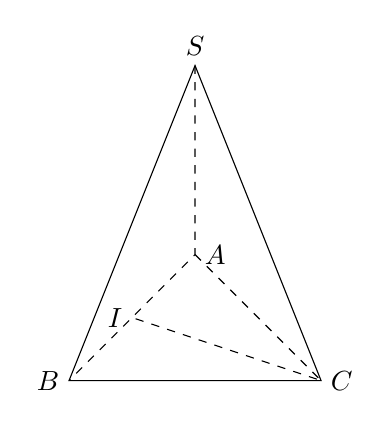
\begin{tikzpicture}[scale=0.8]
					\coordinate (A)  at (0,0);
					\coordinate (B) at  (-2,-2);
					\coordinate (C)  at (2,-2);
					\coordinate (S) at (0,3); 
					\coordinate (I)  at (-1,-1);
					\draw (S) -- (B) -- (C)  -- cycle;
					\draw [dashed] (S) -- (A)  -- (B);
					\draw [dashed] (A) --  (C) -- (I);
					 \fill (A) node[right] {$A$};
					 \fill (B) node[left] {$B$};
					\fill  (C) node[right] {$C$};
					\fill (S) node[above] {$S$}; 
					\fill (I)  node[left] {$I$};
				\end{tikzpicture}
		\end{center}
		\begin{itemchoice}
			\itemch 
			Vì $SA\perp \left(ABC\right)$ nên $A$ là hình  chiếu của $S$ trên $\left(ABC\right)$.
			\itemch 
			Gọi $I$ là trung điểm của $AB$. Vì tam giác $ABC$ là tam giác đều nên $CI\perp AB$. Ta  có $\heva{&{CI\perp AB} \\
			&{CI\perp  SA} \\
			&{SA\cap  AB=A}
			} \Rightarrow CI\perp \left(SAB\right)$. Vậy hình chiếu của  $C$ trên $\left(SAB\right)$ là $I$ với $I$ là trung điểm của $AB$.
			\itemch 
			$SA\perp \left(ABC\right)$  nên $A$ là hình chiếu của $S$ trên $\left(ABC\right)$. Hình chiếu của $B$ lên $\left(ABC\right)$ là $B$, hình chiếu của $C$ lên $\left(ABC\right)$ là $C$. Ta có hình chiếu của tam giác $SBC$ lên $\left(ABC\right)$ là tam giác $ABC$.
			\itemch 
			Vì $CI\perp \left(SAB\right)$ nên hình chiếu của $C$ lên $\left(SAB\right)$ là $I$. Mà hình chiếu của $B$ lên $\left(SAB\right)$ là $B$, hình chiếu của $S$ lên $\left(SAB\right)$ là $S$. Vậy hình chiếu của tam giác $SBC$ trên $\left(SAB\right)$  là tam giác $SIB$.
		\end{itemchoice}
	} 
\end{ex}

% nguồn: Ok_dungsai_lop11_Lan2
\begin{ex}%[1H8H3-3]%[ma:cdf66f24]
	Cho hình chóp $S.ABCD$ có đáy là hình vuông, tam giác  $SAC$ cân và $SA\perp \left(ABCD\right)$. Gọi $H, \; K$ lần lượt là hình chiếu vuông góc của $A$ trên $SB$ và $SC$.
	 \choiceTF
		{\True $AH\perp \left(SBC\right)$} 
		{Góc giữa $AK$ và mặt phẳng $\left(SCD\right)$ bằng  $60^\circ$}
		{Góc giữa $SC$  và mặt phẳng $\left(SAB\right)$ bằng góc $\widehat{SCA}$}
		 {\True Góc tạo bởi $BC$ và $(AHK)$ bằng $30^\circ$}
	 \loigiai{
		\begin{center}
			\begin{tikzpicture}[line cap=round,line join=round,x=1cm,y=1cm]
					 \draw (-2,-1)--(3,-1);
					 \draw (3,-1)--(5,0);
					\draw (-2,-1)--(0,5); 
					\draw (0,5)--(3,-1); 
					 \draw (0,5)--(5,0);
					\draw[dashed] (0,5)--(0,0); 
					\draw[dashed]  (0,0)--(-2,-1);
					\draw[dashed] (5,0)--(0,0); 
					 \draw[dashed] (0,0)--(-1.0159383921863254,1.9521848234410237);
					 \draw[dashed] (-1.0159383921863254,1.9521848234410237)--(2.014770848985729,2.9852291510142717);
					\draw[dashed]  (2.014770848985729,2.9852291510142717)--(0,0);
					\node[below  right] at (0,0) {$A$};
					 \node[below left] at (-2,-1) {$B$};
					 \node[below] at (3,-1) {$C$};
					\node[right] at (5,0) {$D$}; 
					\node[above] at  (0,5) {$S$};
					 \node[left] at (-1.0159383921863254,1.9521848234410237) {$H$};
					\node[right]  at (2.014770848985729,2.9852291510142717) {$K$};
				\end{tikzpicture}
		\end{center}
		\begin{itemchoice}
			\itemch 
			 Ta có $\heva{&BC\perp AB\\
			&BC\perp  SA} \Rightarrow BC\perp \left(SAB\right)$. \\
			Do  $AH\subset \left(SAB\right)$ nên $BC\perp AH$. \\
			Mặt khác, theo giả  thiết $AH\perp SB$. \\
			Từ $BC\perp AH$ và $AH\perp SB$, suy  ra $AH\perp \left(SBC\right)$.
			\itemch 
			Ta có $CD\perp AD$ và $CD\perp SA$ (vì $SA\perp (ABCD)$), suy ra $CD\perp \left(SAD\right)$. \\ 
			Vì $AK$ là hình chiếu vuông góc của $A$  trên $SC$, nên $AK\perp SC$. \\
			Ta có $AK\subset (SAD)$ và  $CD\perp (SAD)$ nên $CD\perp AK$. \\
			Từ $CD\perp AK$ và $AK\perp SC$ ta suy ra $AK\perp (SCD)$ (vì $SC, CD$ là hai đường thẳng  cắt nhau nằm trong mặt phẳng $(SCD)$). \\
			Vậy góc  giữa $AK$ và mặt phẳng $(SCD)$ bằng $90^\circ$.
			\itemch 
			Ta có $BC\perp  AB$ và $BC\perp SA$, suy ra $BC\perp \left(SAB\right)$. \\
			Do $S$ là giao điểm của $SC$ và $\left(SAB\right)$, và $SB$ là hình chiếu của  $SC$ lên $\left(SAB\right)$, nên góc giữa đường thẳng $SC$ và mặt phẳng $\left(SAB\right)$ bằng góc giữa $SC$ và $SB$, chính là góc $\widehat{CSB}$.
			 \itemch
			Ta có  $AH\perp \left(SBC\right)$ và $AK\perp SC$ (theo giả thiết). \\
			Ta cũng có $AH\perp SC$. Do đó, $SC$ vuông  góc với cả hai đường thẳng $AH$ và $AK$. \\
			 Suy ra $SC\perp \left(AHK\right)$. \\
			 Góc tạo bởi đường thẳng $BC$ và mặt phẳng $\left(AHK\right)$ là góc giữa $BC$ và hình chiếu của nó trên mặt phẳng $\left(AHK\right)$. \\
			 Ta có $\left(BC, \left(AHK\right)\right) = 90^\circ - \left(BC, SC\right)$. \\
			Trong tam giác $SBC$  vuông tại $B$ (vì $BC\perp (SAB) \Rightarrow BC\perp SB$), ta có $\tan\left(BC,SC\right) = \tan\widehat{SCB}=\dfrac{SB}{BC}$. \\
			Vì tam giác $SAC$ cân  tại $A$ nên $SA=AC$. Đáy là hình vuông nên $AC=AB\sqrt{2}$. \\
			Do đó  $SA=AB\sqrt{2}$. \\
			Xét tam giác $SAB$ vuông  tại $A$: $SB=\sqrt{SA^2+AB^2}=\sqrt{\left(AB\sqrt{2}\right)^2+AB^2}=\sqrt{2AB^2+AB^2}=AB\sqrt{3}$. \\
			Vậy $\tan  \widehat{SCB}=\dfrac{AB\sqrt{3}}{AB}=\sqrt{3} \Rightarrow \widehat{SCB}=60^\circ$. \\
			Góc tạo bởi  $BC$ và $(AHK)$ là $90^\circ - \widehat{SCB} = 90^\circ-60^\circ=30^\circ$.
		\end{itemchoice}
	} 
\end{ex}
